%%%%%%%%%%%%%%%%%%%%%%%%%%%%%%%%%%%%%%%%%%%%%%%%%%%%%%%%%%%%%%%%%%%%%%%%%%%%%%%%
%2345678901234567890123456789012345678901234567890123456789012345678901234567890
%        1         2         3         4         5         6         7         8

\documentclass[letterpaper, 10 pt, conference]{ieeeconf}  % Comment this line out if you need a4paper

%\documentclass[a4paper, 10pt, conference]{ieeeconf}      % Use this line for a4 paper

\IEEEoverridecommandlockouts                              % This command is only n
\usepackage{amsfonts}
\usepackage{amsmath}
\DeclareMathOperator*{\argmax}{arg\,max}
\usepackage{graphicx}
\graphicspath{ {./figures/} }

\overrideIEEEmargins                                      % Needed to meet printer requirements.

%In case you encounter the following error:
%Error 1010 The PDF file may be corrupt (unable to open PDF file) OR
%Error 1000 An error occurred while parsing a contents stream. Unable to analyze the PDF file.
%This is a known problem with pdfLaTeX conversion filter. The file cannot be opened with acrobat reader
%Please use one of the alternatives below to circumvent this error by uncommenting one or the other
%\pdfobjcompresslevel=0
%\pdfminorversion=4

% See the \addtolength command later in the file to balance the column lengths
% on the last page of the document

% The following packages can be found on http:\\www.ctan.org
%\usepackage{graphics} % for pdf, bitmapped graphics files
%\usepackage{epsfig} % for postscript graphics files
%\usepackage{mathptmx} % assumes new font selection scheme installed
%\usepackage{times} % assumes new font selection scheme installed
%\usepackage{amsmath} % assumes amsmath package installed
%\usepackage{amssymb}  % assumes amsmath package installed
\usepackage{todonotes}

\title{\LARGE \bf Predicting Experienced Presence Exploring Large Mazes in VR}

\author{Lukas Gehrke$^{1}$, Klaus Gramann$^{1,3,4}$% <-this % stops a space
\thanks{This research was supported by a grant from the German Federal Ministry of Education and Research (01GQ1511) to KG}% <-this % stops a space
\thanks{$^{1}$Lukas Gehrke and Klaus Gramann are with Department of Biopsychology and Neuroergonomics, TU Berlin, Strasse des 17. Juni 135, 10623 Berlin, Germany
        {\tt\small lukas.gehrke@tu-berlin.de}}%
\thanks{$^{3}$Center for Advanced Neurological Engineering, University of California San Diego, USA}
\thanks{$^{4}$School of Software, University of Technology Sydney, USA}
}

\begin{document}
\maketitle
\thispagestyle{empty}
\pagestyle{empty}
%%%%%%%%%%%%%%%%%%%%%%%%%%%%%%%%%%%%%%%%%%%%%%%%%%%%%%%%%%%%%%%%%%%%%%%%%%%%%%%%

\begin{abstract}
% must be between 150 and 250, so aiming for 200!
\begin{abstract}
The use of head-mounted virtual reality (VR) to induce presence in a computer simulated world has proven to significantly increase the ecological validity of this medium. In VR, illusions of various kinds (place illusion, plausibility illusion, etc.) occur at the same time for the user to feel present. Most prominently, the embodiment illusion has proven to elicit 'realistic' behavioral as well as physiological responses, when a strong emotional stimulus such as virtual hurting of an embodied rubber hand is provided. Yet, to be able to employ VR and claim ecological validity for less emotional stimuli, the level of presence must be accounted for. We show that the level of presence impacts free spatial exploration behavior in a large scale VR navigation paradigm. Here, we investigate the impact of an established presence metric on ongoing motor behavior demonstrating an analysis framework with a high spatial resolution. We observed participants with higher presence to stay closer to the walls while exploring invisible mazes. Ultimately, we link presence to individual differences in video game experience, sex, and spatial perspective taking abilities, confirming that user characteristics are a defining part of the presence construct.
\end{abstract}
% in the end use hemingway app (http://www.hemingwayapp.com) to increase readability
% Word count is 194:
\end{abstract}

\section{Introduction}
investigate the influence of subjectively reported presence on body movements in VR


\section{Methods}
\indent \textbf{Participants.} Thirty-two healthy participants (aged 21--45 years, 14 men) took part in the
experiment. All participants gave written informed consent to participation and the experimental protocol was approved by the local ethics committee (protocol: GR\_08\_20170428). Three participants were excluded from data analysis due to incomplete data or difficulties in complying with the task requirements.

\indent \textbf{The Invisible Maze Task.} Participants freely explored an interactive sparse invisible maze environment by walking and probing for virtual visual wall feedback with their hand, delivered by a virtual reality (VR) headset. Four different mazes (Fig. \ref{imt_task} B) were explored in three consecutive runs. Upon collision of the hand with an invisible wall, an illuminated white disc was displayed 30cm behind the collision point parallel to the invisible wall (Fig. \ref{imt_task} C). Due to the complexity of the technical details, please consult~\cite{gehrke2018}. In summary, the task required participants to explore mazes to build a spatial representation of the maze layout.%This behavior is comparable to explorative wall touches in the dark to find your way.

\begin{figure}[h]
\centering
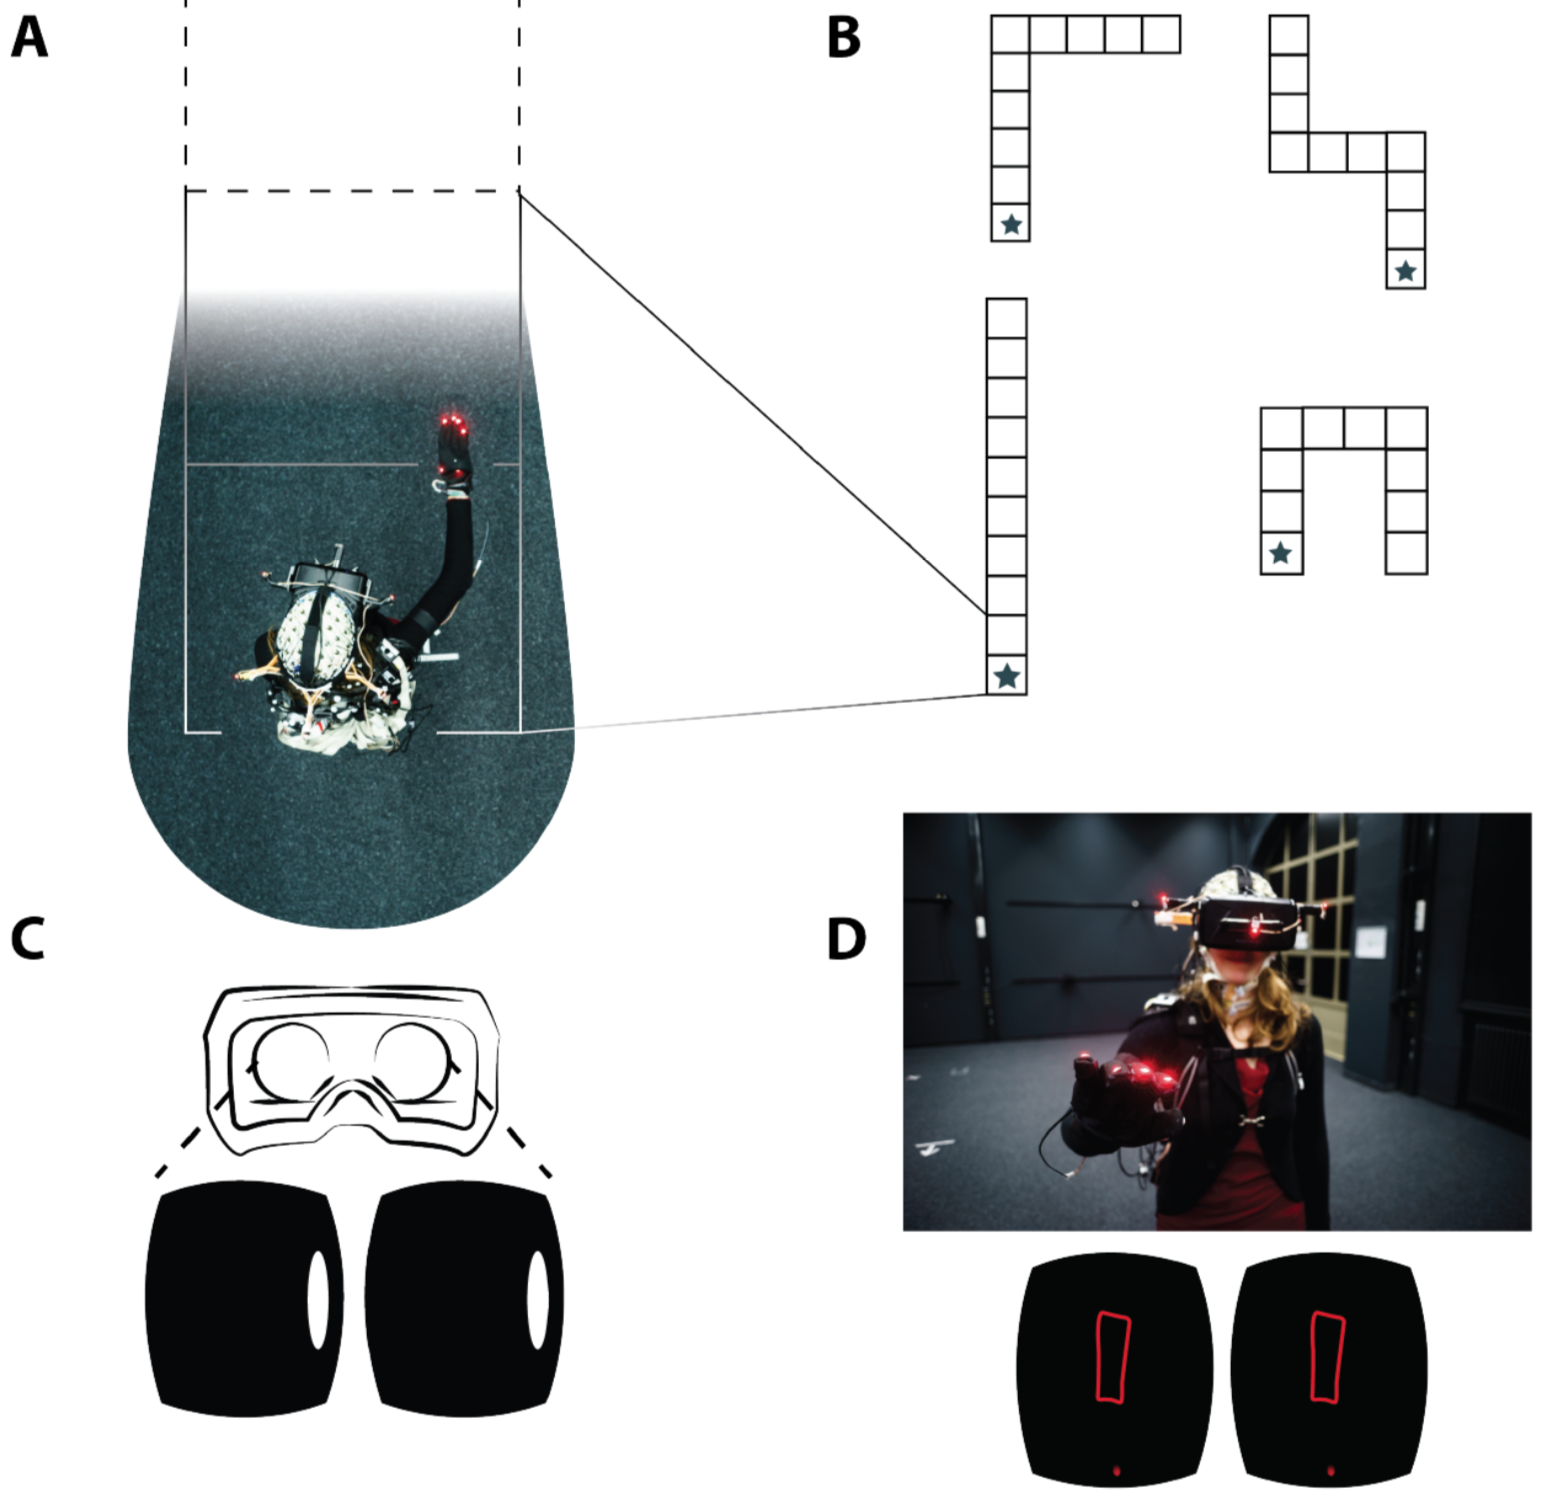
\includegraphics[width=\linewidth]{IMT_Task.png}
\vspace{0pt}
\caption{Invisible Maze Task, \textbf{A} Participant from a bird’s eye view. \textbf{B} Participants are instructed to explore four different mazes and return to the start. \textbf{C} First-person view in binocular ""VR optics"" of a wall touch. \textbf{D} Top: Participants draw a top-down view of the explored maze. Participant is equipped with 160 channels wireless EEG, head-mounted virtual reality goggles and LEDs for motion capture. Bottom: drawn sketch map. Find a detailed description in~\cite{gehrke2018}.}
\label{imt_task}
\end{figure}

\indent \textbf{Assessing experienced presence.} In the current work, we were interested in the subjectively reported experience of presence. Therefore we analyzed the first item on Igroup's presence questionnaire, i.e. 'In the computer generated world I had a sense of "being there"' rated from 'not at all' to 'very much'~\cite{ipq, slaterQ1}.

\indent \textbf{Statistical Analyses.} We computed an ordinary least squares regression entering IPQ presence score as the dependent variable using R~\cite{rver}. For the predictors, we first computed the participant average and then entered: movement velocity, time-on-task, number of wall touches, sketch map accuracy, video game experience, sex, perspective taking and orientation ability, sense of direction into the regression model. For an explanation of each predictor, pleas consult~\cite{gehrke2018}. To reduce over-fitting and increase the possible insight of our results for other researcher, a stepwise model selection procedure based on Akaike's information criterion (AIC) was computed using 'stepAIC' of package 'MASS'~\cite{aic, mass}.
Ultimately, the reduced model of three predictors was assessed in terms of the predictive accuracy of the model. Therefore, a cross-validation with 5 folds was computed to obtain a robust mean absolute error~\cite{cv, mae}. With 29 participants comprising the analyzed data, each training fold consisted of either 23 or 24 participants with either 5 or 6 participants in the evaluated test fold.

% The code and data are available online \todo{add link to data repository and analyses code}


\section{Results}
stepwise regression with IPQ Presence scale as well as IPQ Spatial Presence scale

interesting:
spatial presence is best predicted by time on task and the sketchmaps, whereas general presence is best predicted by video game experience and sex (there is evidence of sex and videogame influence in slater work etc.). Interestingly, in our experiment video game experience negatively impacts presence reported on the general item of the IPQ. This may be due to the overly simplistic visuals of the virtual world. Participants with significant video gaming experience might perceive the world as too artificial.

explore exit interviews and use in discussion!

\section{Discussion}
presence and accuracy of motor behavior, problem because non-continouous metric, cite myself, moderated by learning/difficulty, clustering approaches

presence is best predicted by video game experience and sex (there is evidence of sex and videogame influence in slater work etc.). Interestingly, in our experiment video game experience negatively impacts presence reported on the general item of the IPQ. This may be due to the overly simplistic visuals of the virtual world. Participants with significant video gaming experience might perceive the world as too artificial.

explore exit interviews and use in discussion!

\indent \textbf{Disentangling Presence.}

Sense of ownership, sense of agency etc.

\indent \textbf{Outlook.}

Increasing the resolution of the investigation to finely resolved analysis in space. Motion capture allows us to do that.

% put first image of heatmaps of location and then hint at using mass-univariate regression on each point to increase the resolution of the investigative lens

%%%%%%%%%%%%%%%%%%%%%%%%%%%%%%%%%%%%%%%%%%%%%%%%%%%%%%%%%%%%%%%%%%%%%%%%%%%%%%%%
\addtolength{\textheight}{-12cm}   % This command serves to balance the column lengths
                                  % on the last page of the document manually. It shortens
                                  % the textheight of the last page by a suitable amount.
                                  % This command does not take effect until the next page
                                  % so it should come on the page before the last. Make
                                  % sure that you do not shorten the textheight too much.

%%%%%%%%%%%%%%%%%%%%%%%%%%%%%%%%%%%%%%%%%%%%%%%%%%%%%%%%%%%%%%%%%%%%%%%%%%%%%%%%

\input{bibliography.bib}
\end{document}